
%%%%%%%%%%%%%%%%%%%%%%% file typeinst.tex %%%%%%%%%%%%%%%%%%%%%%%%%
%
% This is the LaTeX source for the instructions to authors using
% the LaTeX document class 'llncs.cls' for contributions to
% the Lecture Notes in Computer Sciences series.
% http://www.springer.com/lncs       Springer Heidelberg 2006/05/04
%
% It may be used as a template for your own input - copy it
% to a new file with a new name and use it as the basis
% for your article.
%
% NB: the document class 'llncs' has its own and detailed documentation, see
% ftp://ftp.springer.de/data/pubftp/pub/tex/latex/llncs/latex2e/llncsdoc.pdf
%
%%%%%%%%%%%%%%%%%%%%%%%%%%%%%%%%%%%%%%%%%%%%%%%%%%%%%%%%%%%%%%%%%%%


\documentclass[runningheads,a4paper]{llncs}

\usepackage{amssymb,amsmath}
\setcounter{tocdepth}{3}
\usepackage{graphicx}

\usepackage{url}
\urldef{\mailsa}\path|{alfred.hofmann, ursula.barth, ingrid.haas, frank.holzwarth,|
\urldef{\mailsb}\path|anna.kramer, leonie.kunz, christine.reiss, nicole.sator,|
\urldef{\mailsc}\path|erika.siebert-cole, peter.strasser, lncs}@springer.com|
\newcommand{\keywords}[1]{\par\addvspace\baselineskip
\noindent\keywordname\enspace\ignorespaces#1}

\begin{document}

\mainmatter  % start of an individual contribution

% first the title is needed
\title{Optimization of Drop Characteristics in a Carrier Cooled Gas Stream
using ANSYS and Globalizer Software Systems on the PNRPU High-Performance
Cluster\thanks{This study was supported by the Russian Science Foundation,
project No. 16-11-10150.}}

% a short form should be given in case it is too long for the running head
\titlerunning{Optimization of Drop Characteristics in a Carrier Cooled Gas Stream}

\author{Stanislav L. Kalyulin (ORCID 0000-0002-5998-0950)$^1$ \and
Evgenya V. Shavrina$^1$ \and
Vladimir Ya. Modorskii (ORCID 0000-0002-4200-3440)$^1$ \and \\
Konstantin A. Barkalov (ORCID 0000-0001-5273-2471)$^2$ \and
Victor P. Gergel (ORCID
0000-0002-4013-2329)$^2$}
%
\authorrunning{S.L. Kalyulin \and E.V. Shavrina \and V.Ya. Modorskii \and K.A. Barkalov \and V.P. Gergel}
% (feature abused for this document to repeat the title also on left hand pages)

% the affiliations are given next; don't give your e-mail address
% unless you accept that it will be published
\institute{$^1$Perm National Research Polytechnical University, Perm, Russia\\
\email{\{ksl, modorsky\}@pstu.ru}\\
$^2$Lobachevsky State University of Nizhny Novgorod, Nizhny Novgorod, Russia\\
\email{\{konstantin.barkalov, victor.gergel\}@itmm.unn.ru}
}

%
% NB: a more complex sample for affiliations and the mapping to the
% corresponding authors can be found in the file "llncs.dem''
% (search for the string "\mainmatter" where a contribution starts).
% "llncs.dem" accompanies the document class "llncs.cls".
%

%\toctitle{Lecture Notes in Computer Science}
%\tocauthor{Authors' Instructions}
\maketitle

\begin{abstract}
We describe in this article the optimization calculations of spray
droplets in a gas injected through a nozzle into a work area, as a part of
a research of icing on model objects in a small-size climatic wind tunnel.
Calculations were performed in a 3D-statement. It is assumed that the drop
has some speed, temperature and diameter as it enters the gas flow, which
has a specified speed and temperature, so that definite temperature limits
are attained when it interacts with a remote obstruction. We determined
the maximum gas flow temperature, which corresponds to the minimum of
cooling energy consumption. The optimization was carried out using the
Globalizer software (Lobachevsky State University of Nizhny Novgorod).
Also, we could solve the integration issue between Globalizer and ANSYS
Workbench 13.0. ANSYS was employed as a tool to calculate optimization
criteria values, whereas Globalizer was used as an optimal parameter
search tool. Calculations were performed on the PNRPU high-performance
cluster (with a peak performance of 24 TFLOPS).

\keywords{small-size climatic wind tunnel, global optimization, multiextremal
functions, parallel algorithms, droplets flying, numerical simulation, gas
flow.}
\end{abstract}

\section{Introduction}

An energy-efficient \cite{Shmakov2016} closed-loop small-sized climatic wind
tunnel (CWT) is being developed at Perm National Research Polytechnical
University (PNRPU) \cite{Modorskii_1_2016} with a view to continue scientific
investigations into the field of aircraft aerodynamics. This installation which
will provide an opportunity to conduct aerodynamic experiments with simulated
in-flight icing conditions at flow Mach numbers as high as $M=0.8$ and
stagnation temperatures up to 30$^\circ$C \cite{Kalyulin2016}.

As it is known, tests in wind tunnels can help to solve the following problems
\cite{Afanasiev1994}:

\begin{enumerate}
\item Investigation of the influence of the gas-streamlined object shape on
    the object aerodynamic characteristics depending on flow velocity and
    the body position in space.

\item Investigation of air machines: gas turbines, compressors, propellers,
    windmills, fans, etc.

\item Investigation of engine characteristics (piston turbojet, ramjet,
    etc.).

\item Investigation of aircraft flight dynamics.

\item Investigation of the influence of aerodynamic forces on the
    elasticity of aircraft structures (e.g., research into aircraft wing
    flutter).

\item Physical investigations related to air flow under different
    conditions (research into the boundary layer, supersonic flows, spatial
    streams, etc.).

\item Methodical and scientific investigations related to the creation of
    wind tunnels as physical facilities, test method development in tunnels
    and processing of the results obtained.
\end{enumerate}

The article discusses the design of an energy-efficient closed-loop small-sized
CWT for full-scale icing simulation. The modeling of this process requires
structural elements such as air-cooling system, injectors for water supply to
the tunnel, a device to heat them, and a dehumidifying system (described in the
patent \cite{Goryachev2007}).

A distinctive feature of the design is its high energy efficiency, which will
allow for testing under icing conditions at a much lower cost than already
existing large testing facilities. This economy is achieved through its ability
to consume only the energy required in operating mode to maintain a
predetermined level of air flow and by reducing the characteristic dimensions
of the CWT \cite{Kalyulin2016}.

According to studies by Russian scientists \cite{Klemenkov2008}, the
contour of the CWT must be open, so that moisture does not accumulate. The
working part is enclosed as its length is enough to equalize the drop
temperature to air temperature. Owing to the fact that large CWTs are
energy-intensive installations, small-size models are becoming more
popular. However, scale model sizes less than $1:8$ lead to distortion of
the icing shape, which is unacceptable. Thus, there is a limitation on the
minimum diameter of the CWT.

Given the large time and material costs that are necessary for the
preparation and execution of physical experiments in an energy-efficient
closed-loop small-sized CWT, numerical simulation of experiments has
become the most popular method for studying icing processes. We propose
the joint use of numerical and physical experiments.

Ice formation processes during field experiments (spraying water with
subsequent freezing) determine three tasks that must be accomplished for the
numerical simulation of processes occurring in a CWT:
\begin{enumerate}
\item Simulation of cooling gas flowing in the CWT.

\item Simulation of drop disintegration to determine correctly the size of
    ice particles.

\item Simulation of the ``water-ice'' phase transition.
\end{enumerate}

ANSYS CFX numerical experiments concerning spraying of water particles are
possible with the use of different mathematical models of various degrees of
accuracy. In most cases, however, significant computational resources are
required.

A modeling of icing was performed in \cite{Alekseenko2013}, but the method
suggested by the authors does not allow to model the characteristics of
the surface roughness, nor complex-shaped ice build-ups (such as the
unevenness of the ``lobster tail'') in icing areas at small slip angles of
the drops. According to \cite{Prihodko2014}, small build-ups of this kind
have a more significant impact than the ``horn-shaped'' ones. Also, that
paper discusses a technique that allows to estimate the probability of
such ice build-ups. It is not possible, however, to obtain sufficiently
accurate data on the nature of the build-ups in such processes as flow
separation from a wing.

Icing simulation in ANSYS FENSAP-ICE has not gained much popularity due to
requirements to conclude additional license agreements and an insufficient
number of validation studies. Nevertheless, a solution example of the
problem of icing in ANSYS FENSAP-ICE in conjunction with ANSYS CFX was
presented by researchers from Louisiana in \cite{Hannat2014}. ANSYS CFX
and ANSYS FLUENT gas dynamics packages are usually used in this regard in
research practice.

As a rule, information on temperature, humidity, speed and other gas
dynamics parameters are used to predict icing,  since a direct modeling of
the ``water-ice'' phase transition is not possible in these packages.
Besides, investigations on gas dynamics problems performed abroad with the
use of the ANSYS CFX and ANSYS FLUENT packages relied on subsequent
accurate gas dynamics parameters to solve the problem of icing by
semi-empirical or analytical methods \cite{Villalpando2016}.

The statement of the problem of numerical simulation depends on the type
of icing, which can be divided into four categories
\cite{Klemenkov2008,Lynch2001,Bragg2005}:

\begin{enumerate}
\item The roughness of the ice surface surpasses the height of the
    local boundary layer, affecting not only the transition of the
    boundary layer to a turbulent state, but also its separation
    downstream.

\item The icing is characterized by grooves along the stream. In this
    case, the area of flow separation primarily depends on the attack
    angle. In combination with its roughness, this type of icing
    mainly affects the increase in resistance.

\item In some cases, the droplets spreading over the surface
    crystallize immediately. Then the ice begins to grow in a vicinity
    of the critical point adopting the shape of a ``horn''. In other
    cases, crystallization is delayed; a film of water creeps over the
    surface, and ice forms along two areas on the side of the critical
    point, forming two ``horns''. The icy ``horns'' create a large
    separated region which affects aerodynamics. This is accompanied
    by the separation of flow depending on their shape, position, and
    angle of attack. It significantly reduces the aircraft�s
    load-bearing properties.

\item When a thermal anti-icing system is working, a film of water
    moves across the surface to the outer boundary of the heated
    region and then freezes in the form of a so-called barrier ice. An
    obstacle is formed which leads to the appearance of a large
    separated region in front and behind. This significantly affects
    the aerodynamic characteristics depending on the position and
    geometry of the obstacle \cite{Bragg2005}.
\end{enumerate}

The nature of these phenomena and the conditions producing a particular
type of icing have not been thoroughly studied until now.

Furthermore, the estimation of the surface tension of small droplets with
a typical diameter of 20~$\mu$m have shown that the excess pressure, which
could affect the freezing point of water and the crystallization process,
is so small that it practically does not affect the freezing temperature
of water \cite{Klemenkov2008}. The surface tension only has an effect on
the spreading of drops when they hit the surface and the disintegration of
the liquid into drops at being expelled from the injectors
\cite{Modorskii_2_2016}. These processes are poorly understood and will be
the subject of forthcoming experimental studies in CWT.

In this regard, mathematical modeling of icing at the moment is not
perfect. Therefore, physical experiments cannot be completely excluded
from consideration. Thus, to maximize at present the effectiveness of
research into icing processes, both numerical and physical experiments are
equally needed.

Investigations are frequently limited to finding one or several solutions
that satisfy the requirements of technical specifications. Searching for
an optimal solution is usually not possible, since it requires  large
computational resources.

Therefore, the numerical search for optimal solutions in an acceptable
time frame is one of the most important tasks
\cite{Gaynutdinova2015,Modorskii_3_2016}. It increases the quality of
decisions and enhances the benefits of numerical calculations, enabling
the identification of new dependencies.

\section{Gas dynamics problem}

\subsection{A physical model of the gas dynamics problem}

In the physical statement of the problem, it is assumed that a drop with a
given velocity, temperature and diameter falls into a gas dynamic flow
having some speed and temperature, so that, upon contact with a distant
obstacle, certain temperature limits are attained \cite{Modorskii2002}.
The distance to the obstacle is equal to 2~m. The maximum temperature of
the carrying gas dynamic flow is determined, and it corresponds to the
minimum energy consumption of the energy-efficient closed-loop small-sized
CWT when it cools.

The calculation is carried out in a 3D dynamic statement. The internal CWT
volume is modeled, and the two-phase environment, gravity and interaction
with the cooling gas dynamic flow are taken into account.

\subsection{Mathematical model of the gas dynamics problem}

We applied the finite volume method for the numerical simulation of the
drop flight from the site of injection through the nozzle to the working
area of the CWT. This implies that the field of the gas dynamic flow is
approximated by a finite number of calculation points.

A mathematical model is developed in accordance with the adopted physical
model. This model is based on the mass, momentum and energy conservation
laws, and is closed with the state equations of an ideal compressible gas
and turbulence, as well as with initial and boundary conditions. The
mathematical model of the gas dynamics problem includes the following
relations \cite{Kozlova2010}:
\begin{itemize}
\item[$\bullet$] The equation of mass conservation for the gas:
\begin{equation}
\frac{\partial}{\partial t}(\rho_{\text{air}})+\bar{\nabla}\cdot(\rho_{\text{air}} V_{\text{air}})=Q^{\text{drop}}_{\text{mass}},
\end{equation}
where $\rho_{\text{air}}$ is the air density, $V_{\text{air}}$ is the
air velocity vector, and $Q^{\text{drop}}_{\text{mass}}$ is a source
term expressing the increase in weight caused by evaporation of water
from the drop surface.

\item[$\bullet$] The equation of momentum conservation for the gas:
\begin{equation}
\frac{\partial}{\partial t}(\rho_{\text{air}} V_{\text{air}})+(\rho_{\text{air}} V_{\text{air}}\cdot \bar{\nabla})\cdot V_{\text{air}}=-\bar{\nabla}P+\bar{\nabla}\tau_{\text{air}}+\rho_{\text{air}}g+Q^{\text{drop}}_{\text{force}},
\end{equation}
where $P$ is pressure, $g$ is the gravity vector, $\tau_{\text{air}}$
is the shear stress at the wall, and $Q^{\text{drop}}_{\text{force}}$
is a source term that expresses the force with which the drop acts on
the air.

\item[$\bullet$] The equation of energy conservation for the gas:
\begin{equation}
\frac{\partial}{\partial t}(\rho_{\text{air}} H_{\text{air}})+\bar{\nabla}\cdot(\rho_{\text{air}} V_{\text{air}} H_{\text{air}})=\frac{\partial P}{\partial t}\cdot\bar{\nabla}\cdot \left(\left(\frac{\lambda_{\text{air}}}{c_{p_{\text{air}}}}+\mu_t\right)\bar{\nabla}H_{\text{air}}\right)+Q^{\text{drop}}_{\text{energy}},
\end{equation}
where $H_{\text{air}}$ is the total enthalpy of the air,
$\lambda_{\text{air}}$ is the coefficient of thermal conductivity of
the air, $c_{p_{\text{air}}}$ is the air heat capacity, $\mu_t$ is
turbulent dynamic viscosity, $Q^{\text{drop}}_{\text{energy}}$ is a
source term expressing energy transfer between the phases.

\item[$\bullet$] The equation of mass conservation for the steam:
\begin{equation}
\frac{\partial}{\partial t}(\rho_{\text{air}} Y_{\text{steam}})+\bar{\nabla}\cdot(\rho_{\text{air}} V_{\text{air}} Y_{\text{steam}})=\bar{\nabla}\cdot\left( \left( \rho_{\text{air}} D + \frac{\mu_t}{S_{c_t}}\right)\bar{\nabla} Y_{\text{steam}}\right)+Q^{\text{drop}}_{\text{mass}},
\end{equation}
where $Y_{\text{steam}}=1-Y_{\text{air}}$ is steam mass concentration,
$Y_{\text{air}}$ is air mass concentration, $D$ is the diffusion
coefficient, and $S_{c_t}$ is the Schmidt turbulent number
($S_{c_t}=1$).

\item[$\bullet$] The equation of state:
\begin{equation}
P=\frac{\rho_{\text{air}}R_0 T_{\text{air}}}{M},
\end{equation}
where $R_0=8314.41~\text{J}/\text{kmol}\cdot \text{K}$ is the
universal gas constant, $M$ is the molecular weight, and
$T_{\text{air}}$ is the air temperature.

\item[$\bullet$] The equation of the drop motion dynamics:
\begin{equation}
\frac{\partial V_{\text{drop}}}{\partial t}=\frac{\pi d^2_{\text{drop}}}{8 m_{\text{drop}}}C_D\rho_{\text{drop}}|V_{\text{air}}-V_{\text{drop}}|(V_{\text{air}}-V_{\text{drop}})+g\left(1-\frac{\rho_{\text{air}}}{\rho_{\text{drop}}}\right),
\end{equation}
where $d_{\text{drop}}$ is the drop diameter, $m_{\text{drop}}$ is the
drop weight, $\rho_{\text{drop}}$ is the drop density,
$V_{\text{drop}}$ is drop velocity, and $C_D$ is the coefficient of
resistance.

\item[$\bullet$] The equation of mass conservation for the drop:
\begin{equation}
\frac{\partial m_{\text{drop}}}{\partial t}=-m^*\pi d^2_{\text{drop}},
\end{equation}
where $m^*$ is the steam injection parameter per drop surface unit.

\item[$\bullet$] The equation of energy conservation for the drop:
\begin{equation}
\frac{\partial T_{\text{drop}}}{\partial t}=\left(\left[\mathrm{Nu}\frac{\lambda_{\text{air}}}{d_{\text{drop}}}(T_{\text{air}}-T_{\text{drop}})\right]-m^* q(T_{\text{drop}})\right)\frac{6}{d_{\text{drop}}\rho_{\text{drop}}c_{p_{\text{drop}}}},
\end{equation}
where $c_{p_{\text{drop}}}$ is the drop heat capacity,
$T_{\text{drop}}$ is the drop temperature, and $\mathrm{Nu}$ is the
Nusselt number.

\item[$\bullet$] The equation of turbulent energy:
\begin{equation}
\frac{\partial}{\partial t}(\rho_{\text{air}}K)+\bar{\nabla}\cdot(\rho_{\text{air}} V_{\text{air}}K)=\bar{\nabla}\cdot\left(\left(\mu+\frac{\mu_t}{\sigma}\right)\bar{\nabla}K\right)+\mu_t G-\rho_{\text{air}}\varepsilon,
\end{equation}
where $\sigma$ is a constant, $G$ determines the speed of turbulent
energy generation, $\varepsilon$ is the rate of turbulent energy
dissipation, and $K$ is turbulent energy.

Given that the computational domain has a cylindrical geometry, the
gas dynamic flow has a high speed, and the length is small and equals
the distance from the injection of droplets through the nozzles to the
barrier (experimental model), it is advisable to use the
$K-\varepsilon$ turbulence model, which is applicable when the
influence of inertial forces is large compared to viscosity forces.

\item[$\bullet$] The equation of turbulent energy dissipation rate:
\begin{equation}
\frac{\partial}{\partial t}(\rho_{\text{air}}\varepsilon)+\bar{\nabla}\cdot(\rho_{\text{air}} V_{\text{air}}\varepsilon)=\bar{\nabla}\cdot\left(\left(\mu+\frac{\mu_t}{\sigma_\varepsilon}\right)\bar{\nabla}\varepsilon\right)+C_1 \frac{\varepsilon}{K}\mu_t G-C_2 f_1 \rho_{\text{air}}\frac{\varepsilon^2}{K},
\end{equation}
where $\sigma_\varepsilon$, $C_1$ and $C_2$ are  constants.
\end{itemize}

\subsection{Parameters and criteria for optimization of gas dynamics calculation}

The problem is solved in ANSYS CFX, as the initial and boundary conditions
are given. We studied the solution convergence. Next, input and output
parameters were parameterized in CFX and transferred to the ANSYS
Workbench, a step that was necessary for the iterative start of ANSYS in
the Globalizer optimization program.

The following ranges of input parameters were set:
\begin{enumerate}
\item $T_{\text{air}}=- 30$ .. $0\,^\circ $C for gas dynamic flow
    temperature;

\item $V_{\text{air}}= $ 10 .. 270~m/s for gas dynamic flow rate;

\item $T_{\text{drop}}|_{l=0} =+5$ .. $+10 \,^\circ$C for the drop
    temperature at the initial moment of contact with the air flow;

\item $V_{\text{drop}}=  10$ .. $270$~m/s for the drop velocity at the
    initial time of contact with the air flow.
\end{enumerate}

The average drop diameter for injecting was taken equal to 20~$\mu$m, and
did not change during computations.

We adopted the following output criteria for the optimization algorithm:
\begin{enumerate}
\item $T_{\text{drop}}|_{l=0} =-0.5$ .. $+0.5\,^\circ$C for the drop
    temperature at the moment when it reaches the obstacle ($L= 2$~m);

\item $T_{\text{air}}\rightarrow \text{max}$ for the maximum initial
    temperature of the gas dynamic flow.
\end{enumerate}

The input parameter $T_{\text{air}}$ is simultaneously an output criterion
that approaches the maximum.

As we know, when integrating the multi-criteria parallel optimization IOSO
PM program complex with ANSYS, it is possible to set the input parameter
as an output optimization criterion only with additional program code
associated with syntactic IOSO PM parameters, i.e. it is not foreseen
within the core function of the optimization complex.

As regards the drop freezing, the air temperature cannot physically be
above $+0.5\,^\circ$C, otherwise the drop will not be able to cool down to
the temperature defined by the output criterion.

The optimization problem was solved with the generalized global
optimization algorithm implemented in Globalizer. To allow for sorting the
results of the Globalizer�s gas dynamics solution in ANSYS CFX, we wrote
the respective functions, and parameterized the total count time
(TotalTime) and the time step (TimeSteps).

The description of both the optimization algorithm and the Globalizer
program system is given in the next section.

\section{Global optimization with non-convex constraints}

\subsection{Problem statement}

Let us consider the $N$-dimensional global optimization problem
\begin{equation}\label{problem}
\varphi(y^\ast)=\min{\left\{\varphi(y):y\in D, \; g_i(y)\leq 0, \; 1 \leq i \leq m\right\}},
\end{equation}
with search domain
\begin{equation}\label{D}
D=\left\{y\in R^N: -2^{-1}\leq y_j \leq 2^{-1}, 1\leq j \leq N \right\}.
%D=\left\{y\in R^N: a_i\leq y_i \leq b_i, 1\leq i \leq N\right\}.
\end{equation}
This problem statement covers a large class of problems since the hyperinterval
\[%\label{S}
S=\left\{y\in R^N: a_j\leq y_j \leq b_j, 1\leq j \leq N \right\}
\]
can be reduced to the hypercube (\ref{D}) by linear transformation. The
objective function $\varphi(y)$ (henceforth denoted by $g_{m+1}(y)$) and
the left-hand sides $g_i(y), \; 1\leq i \leq m$, of the constraints
satisfy the Lipschitz conditions with constants $L_i, \; 1 \leq i \leq
m+1$, respectively,  and may be multiextremal. It is assumed that the
functions $g_i(y)$ are defined and computable only at the points $y \in D$
satisfying the conditions
\begin{equation}\label{g_k}
g_k(y) \leq 0, \; 1 \leq k < i.
\end{equation}

Employing the continuous single-valued Peano curve $y(x)$
(\textit{evolvent}) that maps the unit interval $[0,1]$ of the $x$-axis
onto the $N$-dimensional domain (\ref{D}), it is possible to find the
minimum in the problem (\ref{problem}) by solving the one-dimensional
problem
\[
\varphi(y(x^\ast))=\min \left\{\varphi(y(x)): x \in [0,1], \; g_i(y(x))\leq 0, \; 1 \leq i \leq m\right\},
\]
where, as it follows from(\ref{g_k}), the functions $g_i(y(x))$ are
defined and computable in the domains
\[
Q_1=[0,1], \; Q_{i+1}=\left\{x \in Q_i : g_i(y(x)) \leq 0 \right\}, \; 1 \leq i \leq m.
\]

These conditions allow for the introduction of a classification of the
points $x \in [0,1]$ according to the number $\nu (x)$ of the constraints
computed at this point. The \textit{index} $\nu(x)$ can also be defined by
the conditions
\[
g_i(y(x)) \leq 0, \; 1 \leq i < \nu, \; g_\nu(y(x))>0,
\]
where the last inequality is inessential if $\nu=m+1$.

The considered dimensionality reduction scheme juxtaposes a
multidimensional problem with lipschitzian functions to a one-dimensional
problem where the corresponding functions satisfy the uniform H{\"o}lder
condition (see \cite{Strongin2000}), i.e.
\[
\left|g_i(y(x'))-g_i (y(x''))\right| \leq H_i \left|x'-x'' \right|^{1/N}, \; x',x''\in [0,1], \; 1\leq i \leq m+1.
\]
Here $N$ is the dimensionality of the initial multidimensional problem and
the coefficients $H_i$ are related with the Lipschitz constants $L_i$ of
the initial problem by the inequalities $H_i \leq 2L_i \sqrt{N+3}$.

Thus, a \textit{trial} at a point $x^k \in [0,1]$ executed at the $k$-th
iteration of the algorithm will consist in the following sequence of
operations:
\begin{itemize}
	\item Determine the \textit{image} $y^k=y(x^k)$ in accordance with
the mapping $y(x)$.

	\item Compute the values $g_1(y^k),...,g_\nu(y^k),$ where the
index $\nu \leq m$ is determined by the conditions
	\[
		g_i(y^k )\leq 0, \; 1 \leq i < \nu, \; g_\nu(y^k)>0, \; \nu \leq m.
	\]
\end{itemize}
The occurrence of the first violation of the constraint terminates the
trial. In the case when the point $y^k$ is a feasible one, i.e. when
$y(x^k)\in Q_{m+1}$, the trial includes the computation of the values of
all the functions of the problems and the index is assumed to be
$\nu=m+1$. The pair of values
\[
\nu=\nu(x^k), \; z^k=g_\nu(y(x^k))
\]
is a \textit{trial result}.

\subsection{Generalized global search algorithm}

The rules that determine the work of the index method are the following.

The first trial is executed at an arbitrary internal point $x_1 \in
(0,1)$. The selection of the point $x^{k+1}, \; k \geq 1,$ of any next
trial is determined by the following rules.

Rule 1. Renumber the points $x^1,...,x^k$ of the preceding trials by the
lower indices in ascending order of coordinate values, i.e.
\[
0=x_0<x_1<\dots <x_k<x_{k+1}=1,
\]
and juxtapose to them the values $z_i=g_\nu(y(x_i)), \; \nu=\nu(x_i), \; 1
\leq i \leq k$, computed at these points. The points $x_0=0$ and
$x_{k+1}=1$ are introduced additionally, while the values $z_0$ and
$z_{k+1}$ are not defined.

Rule 2. Classify the indices $i, \; 1 \leq i \leq k$, of the trial points
according to the number of the problem constraints fulfilled at these
points, by constructing the sets
\[
I_\nu =\left\{i:1 \leq i \leq k, \; \nu=\nu(x_i) \right\}, \; 1 \leq \nu \leq m+1,
\]
containing the numbers of all the points $x_i, \; 1 \leq i \leq k$, with
the same values of $\nu$. The end points $x_0=0$ and $x_{k+1}=1$ are
interpreted as the ones having indices equal to zero. An additional set,
$I_0=\left\{0,k+1\right\}$, corresponds to them.

Determine the maximum value of the index:
\[
M=\max\left\{\nu(x_i), \; 1 \leq i \leq k \right \}.
\]

Rule 3. Compute the current lower estimates,
\[
\mu = \max\left\{ \frac{\left|z_i-z_j\right|}{ (x_i - x_j)^{1/N} }, \; i,j \in I_\nu, \; i>j \right\},
\]
for the unknown H{\"o}lder constants $H_\nu$ of the functions $g_\nu(y),1
\leq \nu \leq m+1$. If a set $I_\nu$ contains less than two elements, or
if $\mu_\nu$ is equal to zero, then assume $\mu_\nu=1$.

Rule 4. For all nonempty sets $I_\nu, \; 1 \leq \nu \leq m+1$, compute the
estimates
\[
z_\nu^\ast = \left\{
   \begin{array}{lr}
     -\epsilon_\nu, & \nu < M,\\
     \min\{ g_\nu(y(x_i): i\in I_\nu \}, & \nu = M,
   \end{array}
\right.
 \]
where the nonnegative numbers $(\epsilon_1,...,\epsilon_m)$ are parameters
of the algorithm.

Rule 5. For each interval ($x_{i-1},x_i), \; 1 \leq i \leq k+1,$ compute
the \textit{characteristics} $R(i)$ :
\[
R(i)=2\Delta_i-4\frac{z_i-z_\nu^\ast}{r_\nu \mu_\nu}, \; \nu=\nu(x_i)>\nu(x_{i-1}),
\]
\begin{equation}%\label{eq:14}
R(i)=\Delta_i+\frac{(z_i-z_{i-1})^2}{r_\nu^2 \mu_\nu^2\Delta_i}-2\frac{z_i+z_{i-1}-2z_\nu^\ast}{r_\nu \mu_\nu}, \;  \nu=\nu(x_i)=\nu(x_{i-1}),
\end{equation}
\[
R(i)=2\Delta_i-4\frac{z_{i-1}-z_\nu^\ast}{r_\nu \mu_\nu}, \; \nu=\nu(x_{i-1})>\nu(x_i),
\]
where $\Delta_i=(x_i - x_{i-1})^{1/N}$. The values $r_\nu > 1, \; 1 \leq
\nu \leq m+1,$ are parameters of the algorithm. An appropriate selection
of $r_\nu$ allows to consider the product $r_\nu \mu_\nu$ as an estimate
of the H{\"o}lder constants $H_\nu, \; 1 \leq \nu \leq m+1$.

Rule 6. Find the interval $(x_{t-1},x_t)$ with the maximum characteristic
\begin{equation}\label{MaxR}
R(t)=\max{\left\{R(i): 1 \leq i \leq k+1\right\}}.
\end{equation}

Rule 7. Make the next trial at the midpoint of the interval
$(x_{t-1},x_t)$ if the indices of the points $x_{t-1}$ and $x_t$  are not
the same, i.e.
\[
x^{k+1} = \frac{x_t + x_{t-1}}{2}, \; \nu(x_{t-1}) \neq \nu(x_t).
\]
Otherwise, make the trial at the point
\begin{equation}%\label{eq:142}
x^{k+1} = \frac{x_t+x_{t-1}}{2} - \frac{\mathrm{sign}(z_t-z_{t-1})}{2r_\nu}\left[\frac{\left|z_t-z_{t-1}\right|}{\mu_\nu}\right]^N, \; \nu=\nu(x_{t-1})=\nu(x_t).
\end{equation}

We may take as termination condition the inequality $\Delta_t \leq
\epsilon$, where $t$ is from (\ref{MaxR}) and $\epsilon>0$ is the
predefined accuracy.

Various modifications of this algorithm and the corresponding theory of
convergence are given in
\cite{Strongin2000,Barkalov2002,Gergel2005,Strongin2013}.

The algorithm considered above is very flexible and allows for an
efficient parallelization for shared memory, for distributed memory, and
for accelerators \cite{Barkalov2010,Barkalov2015,Barkalov2016,Gergel2016}.

\section{Integration of Globalizer and ANSYS Workbench}

This section contains a brief explanation of the Globalizer software
system. The system expands the family of global optimization software that
has been consistently developed at Nizhny Novgorod State University during
the past several years.

The development of the system was based on the generalized global search
algorithm that was described in the previous section. A major advantage of
Globalizer is that the system is designed to solve time-consuming
multiextremal optimization problems. The system efficiently uses modern
high-performance computer systems to obtain the optimal solution within a
reasonable time and at a reasonable cost.

The structural components of the Globalizer are the following blocks.
\begin{itemize}
   \item Block 0 consists of the procedures for computing the function
       values (objective and constraints) for the optimization problem
       that is being solved; this is an external block with respect to
       the Globalizer system.

   \item Blocks 1--3 form the optimization subsystem and solve
       unconstrained (Block 1), constrained (Block 2) and
       multicriteria (Block 3) global optimization problems.

   \item Block 4 is a subsystem for accumulating and processing search
       information.
	
   \item Block 5 contains the dimensional reduction procedures based
       on evolvents; the optimization blocks solve the reduced
       (one-dimensional) optimization problems. Block 5 provides for
       interaction between the optimization blocks and the initial
       multidimensional optimization problem.

   \item Block 6 is responsible for managing the parallel processes
       while performing the global search (determining the optimal
       configuration of parallel processes, distributing the processes
       between computer elements, balancing computational loads,
       etc.).

   \item Block 7 is a common managing subsystem, which fully controls
       the entire computational process when solving global
       optimization problems.
\end{itemize}
In order to integrate Globalizer with ANSYS Workbench 13.0, we need to
provide the call of an external calculator of function values (i.e. ANSYS)
as Block 0. It is necessary to transfer the input parameter values of the
ANSYS Workbench project, update the project and  receive the output
parameter values. The transfer of the parameters between the ANSYS
Workbench and Globalizer was implemented by means of an IronPython script.

In the conducted experiments, computations were performed on a single
cluster node. The parallelization of computations of the problem function
values relied on ANSYS tools. The computation costs of executing the
optimization algorithm in Globalizer (the choice of the next trial points,
processing the trial results, etc.) were significantly less than those  of
computing the problem function values in ANSYS. Therefore, it was not
necessary to parallelize the operations of the optimization module itself.

It is important to note that the integration of ANSYS and Globalizer
allows for larger scale experiments to be performed with the use of
several cluster nodes as well. In this case, search trials at different
points of the search domain will be performed at all the nodes that are
employed at each iteration of the method. Therefore, the results of the
computations can be processed in Globalizer both synchronously and
asynchronously. In the first case, the system waits until the computations
on all nodes employed are completed. Then the processing of the results is
performed, and the next iteration is started. This regime is preferred at
equal computing time at any point of the search domain. In the second
case, the results obtained at one of the nodes are processed immediately,
and the next trial begins at this node. The asynchronous regime provides
for the full load of the nodes to be utilized in the cases when trial
times are different at different points of the search domain. The
experiments performed earlier on test problems have demonstrated this
approach to be promising \cite{Gergel2015}. Performing experiments of this
kind on the solution of applied problems will be the subject of further
investigations.

\section{Optimization results}

The Globalizer system allowed to construct a field of input parameter
values that satisfy the above-mentioned (Sec. 2.3) restrictions of the gas
dynamics problem (Fig.~\ref{fig1}).

The total time spent on finding the solution of the optimization problem
at the PNRPU high-performance computing complex was 48 hours.

\begin{figure}
\centering
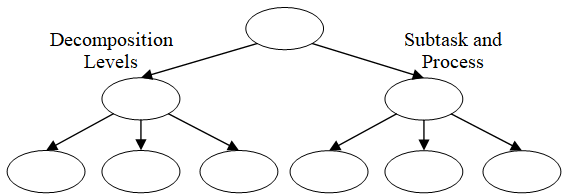
\includegraphics[height=6 cm]{fig1}
\caption {Field of input parameter values that satisfy the output criteria of the
optimization problem: $V_{\text{drop}}$~--- drop velocity, $T_{\text{drop}}|_{l=0}$~---
drop temperature at the time of injection, $V_{\text{air}}$~--- air velocity}
\label{fig1}
\end{figure}

It was assumed that the energy-efficient modes of the CWT are those in
which the gas dynamic flow temperature in the working section approaches
the maximum at the drop temperature $+0.5\,^\circ$C when it reaches the
barrier at a 2~m distance from the injection point:

$T_{\text{air}}\rightarrow \text{max}$;

$T_{\text{drop}}|_{l=2~\text{m}} = 0.5 \,^\circ$C.

However, according to expert estimates, the ranges of permissible drop
speed $V_{\text{drop}}$ and temperature $T_{\text{drop}}|_{l=0}$ at the
time of injection are the following:

$V_{\text{drop}}= $ 5 .. 270~m/s;

$T_{{\text{drop}}|_{l=0}} =+$5 .. $+$10 $^\circ$C.

As the optimization computations show, the values of drop speed and
temperature in the energy-efficient modes of the CWT can vary within the
following ranges (Fig.~\ref{fig1}):

$V_{\text{drop}}= 42.37$ .. 237.63~m/s;

$T_{\text{drop}}|_{l=0} =+5$ .. $+9\,^\circ$C.

An analysis of the results of the computational optimization experiment
(Fig.~\ref{fig1}) showed that the range of drop velocities
$V_{\text{drop}}$ and drop temperatures $T_{\text{drop}}|_{l=0}$
corresponding to these modes of operation is narrower than the recommended
pre-peer evaluations.

These findings identify the speed (for 26.32\%) and temperature (for 20\%)
of the injection modes that produce icing in the work area based at the
specified distance of the experimental model to the injection zone.

Fig.~\ref{fig2} shows that the variation of only two parameters, such as
the speed of the gas dynamic flow ($V_{\text{air}}$) and the drop
temperature at the time of injection through the nozzles
($T_{\text{drop}}|_{l=0}$), allows to achieve the desired value of the
drop temperature ($+0.5\,^\circ$C) upon reaching the barrier (experimental
model) when meeting the output optimization criterion
$T_{\text{air}}\rightarrow+0.5 \,^\circ$C. This may help to achieve
energy-efficient modes in the CWT.

\begin{figure}
\centering
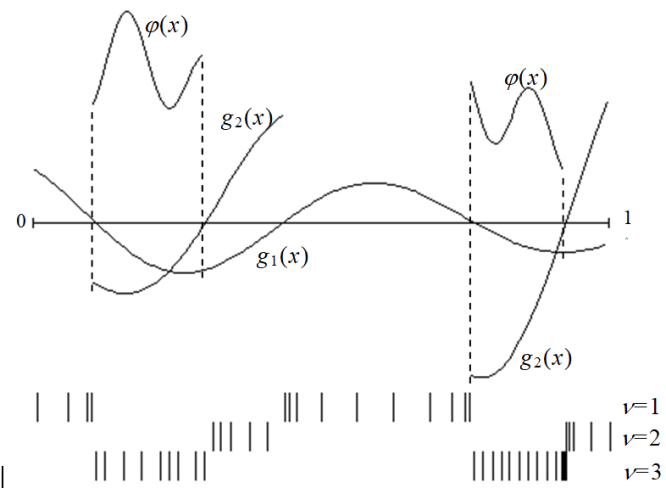
\includegraphics[height=6 cm]{fig2}
\caption {Dependence of $V_{\text{air}}$ (gas dynamic flow rate) and $T_{\text{air}}$
(gas dynamic flow temperature) on $T_{\text{drop}}|_{l=2~\text{m}}$ (drop temperature
when reaching the obstacle ($L= 2$~m)) for different values of $T_{\text{drop}}|_{l=0}$
(drop temperature at time of injection)}
\label{fig2}
\end{figure}

For example, in the given operation mode of the studied experimental
model, by varying only technological parameters such as temperature and
velocity of drops at the initial moment of contact with the gas flow, one
can achieve an energy-efficient simulation of ice formation, except for a
few bottlenecks in the drop velocity modes. Moreover, areas can be
specified by applying a greater number of iterations (ANSYS starts) in the
Globalizer optimization algorithm, which, of course, requires longer
computation times.

\section{Conclusions}

\begin{enumerate}
\item As a result of the solution to the optimization problem, a
    combined region of speed and temperature parameters has been
    detected, as well as the air flow velocity at which the gas
    dynamic flow temperature in the working section approaches the
    maximum. This region is energy efficient, since it allows for
    icing without achieving significant negative airflow temperatures.

\item The possibility of implementing an energy efficient operation
    mode of the small-sized closed-loop CWT has been demonstrated by
    changing only technological parameters such as the initial drop
    temperature and velocity.

\item The integration of the Globalizer optimization system and the
    engineering software package ANSYS has been realized for the first
    time.

\item The Globalizer software package helps to find the best solutions
    at reasonable time and material costs.

\item The application of the Globalizer optimization software system
    made it possible to identify a fairly wide range of parameter
    combinations that allows to maintain the energy-efficient
    operation mode of the small-sized closed-loop CWT with sufficient
    accuracy for engineering practice ($\pm1\,^\circ$C).
\end{enumerate}

\begin{thebibliography}{25}

\bibitem{Modorskii_1_2016}
Modorskii, V.Ya., Shevelev, N.A.: Research of aerohydrodynamic and aeroelastic processes on PNRPU HPC system. In: Vasily Fomin (Ed.) ICMAR 2016, AIP Conference Proceedings, vol. 1770, art. no. 020001 (2016); DOI: 10.1063/1.4963924

\bibitem{Shmakov2016}
Shmakov, A.F., Modorskii, V.Y.: Energy Conservation in Cooling Systems at Metallurgical Plants. Metallurgist 59(9--10), 882--886 (2016); DOI: 10.1007/s11015-016-0188-8

\bibitem{Kalyulin2016}
Kalyulin, S.L., Modorskii, V.Ya., Paduchev, A.P.: Numerical design of the rectifying lattices in a small-sized wind tunnel. In: Vasily Fomin (Ed.) ICMAR 2016, AIP Conference Proceedings, vol. 1770, art. no. 030110 (2016); DOI: 10.1063/1.4964052

\bibitem{Afanasiev1994}
Afanasiev, V.A., Barsukov, V.S., Gofin, M.Ya., Zakharov, Yu.V., Strelchenko, A.N., Shalunov, N.P.: Experimental testing of spacecraft. MAI, Moscow (1994) [in Russian]

\bibitem{Goryachev2007}
Goryachev, A.V., Mezhzil, E.K., Petrov, S.B., Syrov, V.A., Harlamov, A.V., Chivanov, S.V.: A way of ground testing objects of aircraft, subject to icing, and a device for its implementation. Patent RF, no. 2345345 (2007)

\bibitem{Klemenkov2008}
Klemenkov, G.P., Prihodko, Yu.M., Puzyrev, L.N., Haritonov, A.M.: Modelling of aircraft icing processes in aeroclimatic tubes. Thermophysics and Aeromechanics 15(4), 563--572  (2008) [in Russian]

\bibitem{Alekseenko2013}
Alekseenko, S.V., Prihodko, A.A.: Numerical simulation of icing cylinder and profile. Models review and calculation results. TsAGI Science Journal 44(6), 25--57 (2013) [in Russian]

\bibitem{Prihodko2014}
Prihodko, A.A., Alekseenko, S.V.: Numerical simulation of icing aerodynamic surfaces in the presence of large overcooled water drops. JETP Letters 40(19), 75--82 (2014) [in Russian]

\bibitem{Hannat2014}
Hannat, R., Morency, F.: Numerical Validation of Conjugate Heat Transfer Method for Anti-/De-Icing Piccolo System. J. Aircr. 51(1), 104--116 (2014); DOI: 10.2514/1.c032078

\bibitem{Villalpando2016}
Villalpando, F., Reggio, M., Ilinca, A.: Prediction of ice accretion and anti-icing heating power on wind turbine blades using standard commercial software. Energy 114, 1041--1052 (2016); DOI: 10.1016/j.energy.2016.08.047

\bibitem{Lynch2001}
Lynch, F.T., Khodadoust, A.: Effects of ice accretions on aircraft aerodynamics. Prog. Aeosp. Sci. 37(8), 669--767 (2001); DOI: 10.1016/s0376-0421(01)00018-5

\bibitem{Bragg2005}
Bragg, M.B., Broeren, A.P., Blumenthal, L.A.: Iced-airfoil aerodynamics. Prog. Aeosp. Sci. 41(5), 323--362 (2005); DOI: 10.4271/2003-01-2098

\bibitem{Modorskii_2_2016}
Modorskii, V.Ya., Sipatov, A.M., Babushkina, A.V., Kolodyazhny, D.Yu., Nagorny, V.S.: Modeling technique for the process of liquid film disintegration. In: Vasily Fomin (Ed.) ICMAR 2016, AIP Conference Proceedings, vol. 1770, art. no. 030109 (2016); DOI: 10.1063/1.4964051

\bibitem{Gaynutdinova2015}
Gaynutdinova, D.F., Modorsky, V.Y., Masich, G.F.: Infrastructure of Data Distributed Processing in High-Speed Process Research Based on Hydroelasticity Tasks. In: Sloot, P. (Ed.) YSC, Procedia Computer Science, vol. 66, pp. 556--563 (2015); DOI: 10.1016/j.procs.2015.11.063

\bibitem{Modorskii_3_2016}
Modorskii, V.Y., Gaynutdinova, D.F., Gergel, V.P., Barkalov, K.A.: Optimization in Design of Scientific Products for Purposes of Cavitation Problems. In: Simos T.E. (Ed.) ICNAAM 2015, AIP Conference Proceedings, vol. 1738, art. no. 400013 (2016); DOI: 10.1063/1.4952201

\bibitem{Modorskii2002}
Modorskii, V.Y., Sokolkin, Y.V.: Dynamic Behavior of a thick-walled cylinder under pressurization. Izv. Vyss. Uchebnykh Zaved. Aviats. Tek. 4, 14--16 (2002)

\bibitem{Kozlova2010}
Kozlova, A.V., Modorskii, V.Y., Ponik, A.N.: Modeling of Cooling Processes in the Variable Section Channel of a Gas Conduit. Russian Aeronautics 53(4), 401--407 (2010); DOI: 10.3103/s1068799810040057

\bibitem{Strongin2000}
Strongin, R.G., Sergeyev, Y.D.: Global Optimization with Non-Convex Constraints. Sequential and Parallel Algorithms. Kluwer Academic Publishers, Dordrecht (2000); DOI: 10.1007/978-1-4615-4677-1

\bibitem{Barkalov2002}
Barkalov, K.A., Strongin, R.G.: A global optimization technique with an adaptive order of checking for constraints. Comput. Math. Math. Phys. 42(9), 1289--1300 (2002)

\bibitem{Gergel2005}
Gergel, V.P., Strongin, R.G.: Parallel computing for globally optimal decision making on cluster systems. Future Gener. Comput. Syst. 21(5), 673--678 (2005); DOI: 10.1016/j.future.2004.05.007

\bibitem{Strongin2013}
Sergeyev, Ya.D., Strongin, R.G., Lera, D.: Introduction to global optimization exploiting space-filling curves. Springer (2013);  DOI: 10.1007/978-1-4614-8042-6

\bibitem{Barkalov2010}
Barkalov, K., Ryabov, V., Sidorov, S.: Parallel Scalable Algorithms with Mixed Local-Global Strategy for Global Optimization Problems. In: Hsu, Ch., Malyshkin, V. (Eds.) MTPP 2010, LNCS, vol. 6083, pp. 232--240. Springer, Heidelberg (2010); DOI: 10.1007/978-3-642-14822-4$\_$26

\bibitem{Barkalov2015}
Barkalov, K., Gergel, V., Lebedev, I.: Use of Xeon Phi Coprocessor for Solving Global Optimization Problems. In: Malyshkin, V. (Ed.) PaCT 2015, LNCS, vol. 9251, pp. 307--318. Springer, Heidelberg (2015); DOI: 10.1007/978-3-319-21909-7$\_$31

\bibitem{Barkalov2016}
Barkalov, K., Gergel, V.: Parallel Global Optimization on GPU. J. Glob. Optim. 66(1), 3--20 (2016); DOI: 10.1007/s10898-016-0411-y

\bibitem{Gergel2016}
Barkalov, K., Gergel, V., Lebedev, I.: Solving Global Optimization Problems on GPU Cluster. In: Simos T.E. (Ed.) ICNAAM 2015, AIP Conference Proceedings, vol. 1738, art. no. 400006 (2016); DOI: 10.1063/1.4952194

\bibitem{Gergel2015}
Gergel, V., Sidorov, S.: A Two-Level Parallel Global Search Algorithm for Solution of Computationally Intensive Multiextremal Optimization Problems. In: Malyshkin, V. (Ed.) PaCT 2015, LNCS, vol. 9251, pp. 505--515. Springer, Heidelberg (2015); DOI: 10.1007/978-3-319-21909-7$\_$49


%\bibitem{jour} Smith, T.F., Waterman, M.S.: Identification of Common Molecular Subsequences. J. Mol. Biol. 147, 195--197 (1981)

%\bibitem{lncschap} May, P., Ehrlich, H.C., Steinke, T.: ZIB Structure Prediction Pipeline: Composing a Complex Biological Workflow through Web Services. In: Nagel, W.E., Walter, W.V., Lehner, W. (eds.) Euro-Par 2006. LNCS, vol. 4128, pp. 1148--1158. Springer, Heidelberg (2006)

%\bibitem{book} Foster, I., Kesselman, C.: The Grid: Blueprint for a New Computing Infrastructure. Morgan Kaufmann, San Francisco (1999)

%\bibitem{proceeding1} Czajkowski, K., Fitzgerald, S., Foster, I., Kesselman, C.: Grid Information Services for Distributed Resource Sharing. In: 10th IEEE International Symposium on High Performance Distributed Computing, pp. 181--184. IEEE Press, New York (2001)

%\bibitem{proceeding2} Foster, I., Kesselman, C., Nick, J., Tuecke, S.: The Physiology of the Grid: an Open Grid Services Architecture for Distributed Systems Integration. Technical report, Global Grid Forum (2002)

%\bibitem{url} National Center for Biotechnology Information, \url{http://www.ncbi.nlm.nih.gov}

\end{thebibliography}

\end{document}
